% Intended LaTeX compiler: pdflatex
\documentclass[11pt]{article}
\usepackage[utf8]{inputenc}
\usepackage[T1]{fontenc}
\usepackage{graphicx}
\usepackage{longtable}
\usepackage{wrapfig}
\usepackage{rotating}
\usepackage[normalem]{ulem}
\usepackage{amsmath}
\usepackage{amssymb}
\usepackage{capt-of}
\usepackage{hyperref}
\author{Construção de compiladores I}
\date{}
\title{Análise Léxica}
\hypersetup{
 pdfauthor={Construção de compiladores I},
 pdftitle={Análise Léxica},
 pdfkeywords={},
 pdfsubject={},
 pdfcreator={Emacs 29.4 (Org mode 9.7.22)}, 
 pdflang={English}}
\begin{document}

\maketitle
\section*{Objetivos}
\label{sec:org3354a03}

\subsection*{Objetivos}
\label{sec:org3d29198}

\begin{itemize}
\item Apresentar a importância da etapa de análise léxica
em um compilador.
\item Apresentar a implementação de um analisador léxico ad-hoc
para uma linguagem simples.
\end{itemize}
\subsection*{Objetivos}
\label{sec:org7a982b1}

\begin{itemize}
\item Mostrar como a teoria de expressões regulares e autômatos pode ser utilizada para automatizar a criação de analisadores léxicos.
\end{itemize}
\subsection*{Objetivos}
\label{sec:org28a962b}

\begin{itemize}
\item Apresentar o gerador de analisadore léxicos, Alex
\end{itemize}
\section*{Análise léxica}
\label{sec:orge686e10}

\subsection*{Análise léxica}
\label{sec:org103ef9f}

\begin{itemize}
\item Primeira etapa do front-end de um compilador.
\item Simplificar a entrada para análise sintática.
\end{itemize}
\subsection*{Análise léxica}
\label{sec:orge8faadc}

\begin{itemize}
\item Simplificações:
\begin{itemize}
\item Remoção de espaços em branco.
\item Remoção de comentários.
\end{itemize}

\item Resultado: lista de \textbf{\textbf{tokens}}.
\end{itemize}
\subsection*{Análise léxica}
\label{sec:org2277d79}

\begin{itemize}
\item Token
\begin{itemize}
\item Componente indivisível da sintaxe de uma linguagem.
\end{itemize}
\end{itemize}
\subsection*{Análise léxica}
\label{sec:orgecf268d}

\begin{itemize}
\item Exemplos de tokens:
\begin{itemize}
\item identificadores
\item palavras reservadas
\item separadores
\item literais
\end{itemize}
\end{itemize}
\subsection*{Análise léxica}
\label{sec:org31f8918}

\begin{itemize}
\item Como implementar a análise léxica?
\end{itemize}
\subsection*{Análise léxica ad-hoc}
\label{sec:org0240f5c}

\begin{itemize}
\item Percorra a string:
\begin{itemize}
\item Se for um dígito, guarde-o para formar um número.
\item Se for um operador, gere o token.
\item Se for um parêntesis, gere o token.
\item Se for um espaço, tente gerar um número e descarte o espaço.
\end{itemize}
\end{itemize}
\subsection*{Análise léxica ad-hoc}
\label{sec:org94f1434}

\begin{itemize}
\item Como representar tokens?
\end{itemize}

\begin{verbatim}
data Token
  = Number Int
  | Add
  | Minus
  | LParen
  | RParen
  deriving (Eq, Show)
\end{verbatim}
\subsection*{Análise léxica ad-hoc}
\label{sec:orgac0f8de}

\begin{itemize}
\item Configuração do analisador léxico
\begin{itemize}
\item Lista de tokens encontrados.
\item String de dígitos consecutivos encontrados.
\end{itemize}
\end{itemize}

\begin{verbatim}
type LexerState = Maybe ([Token], String)
\end{verbatim}
\subsection*{Análise léxica ad-hoc}
\label{sec:org523ae11}

\begin{itemize}
\item Como finalizar um número?
\begin{itemize}
\item Encontrando um espaço ou operador, criamos um token
com os dígitos.
\end{itemize}
\end{itemize}

\begin{verbatim}
updateState :: LexerState -> LexerState
updateState Nothing = Nothing
updateState ac@(Just (ts, ns))
  | all isDigit ns && not (null ns)
    = let v = read (reverse ns)
      in Just (Number v : ts, [])
  | otherwise =ac
\end{verbatim}
\subsection*{Análise léxica ad-hoc}
\label{sec:org06bc440}

\begin{itemize}
\item Iterando sobre a string de entrada.
\end{itemize}

\begin{verbatim}
lexer' :: LexerState -> String -> LexerState
lexer' ac [] = updateState ac
lexer' Nothing _ = Nothing
lexer' ac@(Just (ts, ns)) (c:cs)
  | isSpace c = lexer' (updateState ac) cs
  | isDigit c = lexer' (Just (ts, c : ns)) cs
  | c == '(' = lexer' (Just (LParen : ts, ns)) cs
  | c == ')' = lexer' (Just (RParen : ts, ns)) cs
  | c == '+' = lexer' (Just (Add : ts, ns)) cs
  | c == '*' = lexer' (Just (Mult : ts, ns)) cs
  | otherwise = Nothing
\end{verbatim}
\subsection*{Análise léxica ad-hoc}
\label{sec:orgf855696}

\begin{itemize}
\item Interface principal do analisador
\end{itemize}

\begin{verbatim}
lexer :: String -> Maybe [Token]
lexer s
  = case lexer' (Just ([], "")) s of
      Nothing -> Nothing
      Just (ts, _) -> Just (reverse ts)
\end{verbatim}
\subsection*{Análise léxica ad-hoc}
\label{sec:org8978284}

\begin{itemize}
\item Algoritmo simples para análise léxica de uma linguagem.

\item Problema: difícil de extender.
\begin{itemize}
\item Como incluir números de ponto flutuante?
\item Como incluir identificadores e palavras reservadas?
\end{itemize}
\end{itemize}
\subsection*{Análise léxica ad-hoc}
\label{sec:orgc80e057}

\begin{itemize}
\item Para acomodar essas mudanças, precisamos de uma abordagem
sistemática para a análise léxica.

\item Para isso, utilizaremos a teoria de expressões regulares
e autômatos finitos.
\end{itemize}
\section*{Expressões regulares}
\label{sec:org95193fa}

\subsection*{Expressões regulares}
\label{sec:orga0404e0}

\begin{itemize}
\item Formalismo algébrico para descrição de linguagens.
\item Amplamente utilizado para representação de padrões em texto.
\item Análise léxica: dividir texto em subpadrões de interesse.
\end{itemize}
\subsection*{Expressões regulares}
\label{sec:org79a8193}

\begin{itemize}
\item Qual a relação entre ERs e análise léxica?
\begin{itemize}
\item Usando ERs podemos \textbf{\textbf{automatizar}} a construção de analisadores léxicos.
\end{itemize}
\end{itemize}
\subsection*{Expressões regulares}
\label{sec:org4164f77}

\begin{itemize}
\item Em essência, um analisador léxico é um AFD que produz
uma lista de tokens.
\item Em Teoria da computação, vimos que toda ER possui um AFD
equivalente
\begin{itemize}
\item Construção de Thompson / derivadas
\end{itemize}
\end{itemize}
\subsection*{Expressões regulares}
\label{sec:org56cdb2f}

\begin{itemize}
\item Construção de Thompson
\begin{itemize}
\item Baseada em propriedades de fechamento de AFs.
\item Cria um AFN com transições lambda.
\end{itemize}
\end{itemize}
\subsection*{Expressões regulares}
\label{sec:org6f42691}

\begin{itemize}
\item Construção de Thompson para lambda.
\end{itemize}

\begin{center}

\includegraphics[width=.9\linewidth]{./Thompson-epsilon.png}
\end{center}
\subsection*{Expressões regulares}
\label{sec:org7975814}

\begin{itemize}
\item Construção de Thompson para símbolo.
\end{itemize}

\begin{center}
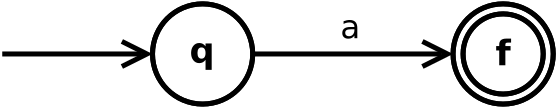
\includegraphics[width=.9\linewidth]{./Thompson-a-symbol.png}
\end{center}
\subsection*{Expressões regulares}
\label{sec:org4a515e7}

\begin{itemize}
\item Construção de Thompson para união.
\end{itemize}
\begin{center}
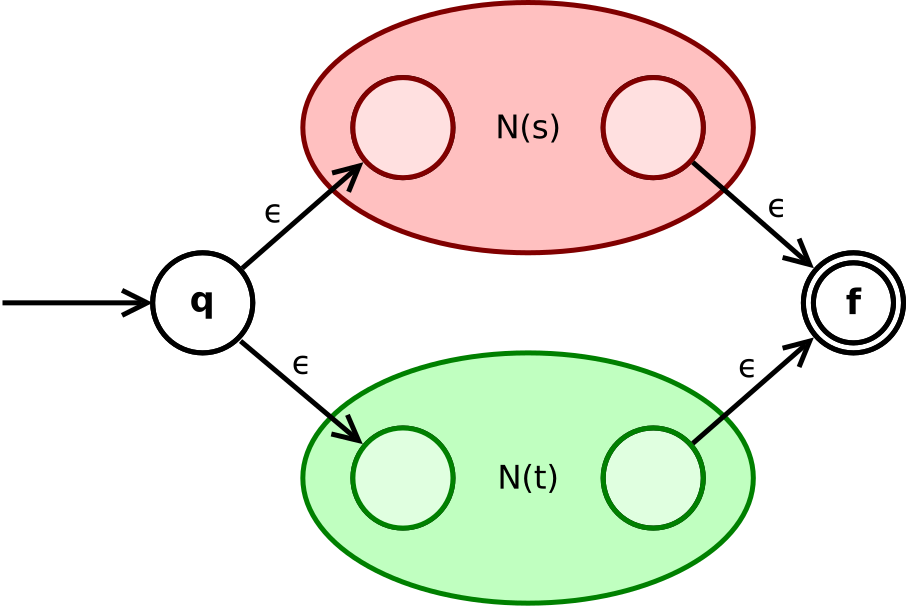
\includegraphics[width=.9\linewidth]{./Thompson-or.png}
\end{center}
\subsection*{Expressões regulares}
\label{sec:org396166b}

\begin{itemize}
\item Construção de Thompson para concatenação.
\end{itemize}

\begin{center}
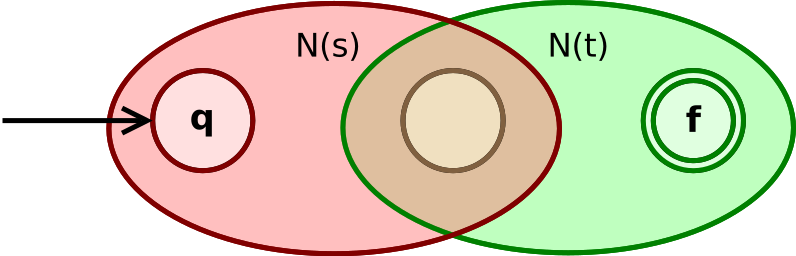
\includegraphics[width=.9\linewidth]{./Thompson-concat.png}
\end{center}
\subsection*{Expressões regulares}
\label{sec:org2ef038b}

\begin{itemize}
\item Construção de Thompson para Kleene.
\end{itemize}

\begin{center}
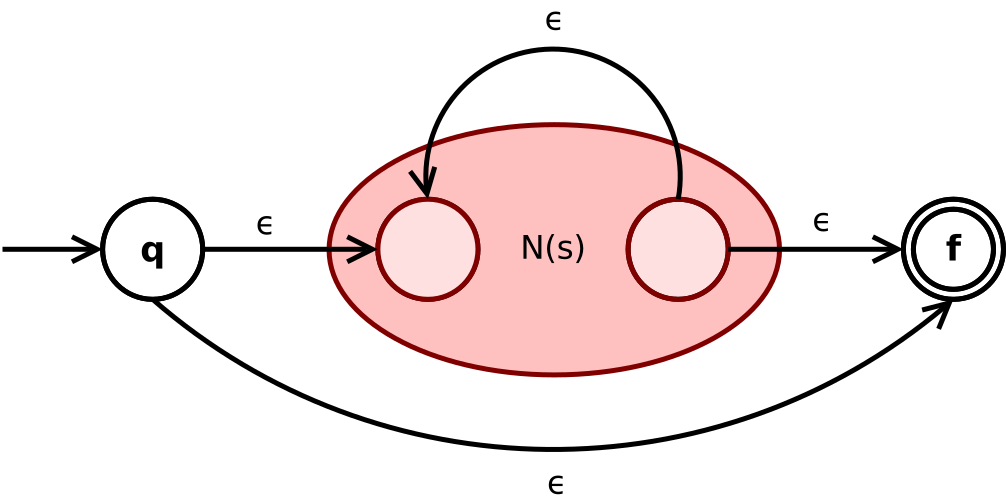
\includegraphics[width=.9\linewidth]{./Thompson-kleene-star.png}
\end{center}
\subsection*{Expressões regulares}
\label{sec:org5a346c2}

\begin{itemize}
\item Como representar AFD em código?
\begin{itemize}
\item Normalmente, utilizamos uma matriz para representar a função de transição.
\end{itemize}
\end{itemize}
\subsection*{Expressões regulares}
\label{sec:org61722ac}

\begin{itemize}
\item Representando um AFD:
\end{itemize}

\begin{verbatim}
-- a: type for states
-- b: type for alphabet symbols

data DFA a b
  = DFA {
      start :: a
    , trans :: [((a,b), a)]
    , final :: [a]
    } deriving Show
\end{verbatim}
\subsection*{Expressões regulares}
\label{sec:org7195ef7}

\begin{itemize}
\item Processando palavras usando o AFD
\end{itemize}

\begin{verbatim}
delta :: (Eq a, Eq b) => DFA a b -> [b] -> Maybe a
delta m s = foldl step (Just (start m)) s
  where
    step (Just e) a
      = lookup (e,a) (trans m)
    step Nothing _ = Nothing
\end{verbatim}
\subsection*{Expressões regulares}
\label{sec:org4eb4da2}

\begin{itemize}
\item Representando o AFD de números:
\end{itemize}

\begin{verbatim}
data State = S0 | S1 deriving (Eq, Show)

numberDFA :: DFA State Char
numberDFA
  = DFA {
      start = S0
    , trans = [((S0, c), S1) | c <- ['0'..'9']] ++
              [((S1, c), S1) | c <- ['0'..'9']]
    , final = [S1]
    }
\end{verbatim}
\subsection*{Expressões regulares}
\label{sec:orgd40782b}

\begin{itemize}
\item Como usar AFDs para produzir os tokens?
\begin{itemize}
\item Crie o token usando o maior prefixo possível processado.
\end{itemize}
\end{itemize}
\subsection*{Expressões regulares}
\label{sec:orge99c4be}

\begin{itemize}
\item Produzindo um token
\end{itemize}

\begin{verbatim}
extract :: DFA State Char -> String -> (String, String)
extract m s = go (start m) "" s
  where
    go _ token [] = (token, [])
    go e token (x : xs)
      | isSpace x = (token, x : xs)
      | otherwise = case lookup (e,x) (trans m) of
                      Just e' -> go e' (token ++ [x]) xs
                      Nothing -> (token, x : xs)
\end{verbatim}
\subsection*{Expressões regulares}
\label{sec:org75c1be1}

\begin{itemize}
\item Analisador léxico
\end{itemize}

\begin{verbatim}
dfaLexer :: DFA State Char -> String -> [Token]
dfaLexer m s = go s []
  where
    go [] ac = reverse ac
    go (x : xs) ac
      | isSpace x = go xs ac
      | otherwise =
        let (token, rest) = extract m (x : xs)
        in go rest (if null token then ac else Number (read token) : ac)
\end{verbatim}
\subsection*{Expressões regulares}
\label{sec:org88c0205}

\begin{itemize}
\item Esse código simples funciona para apenas um AFD.

\item A especificação de uma linguagem é formada por várias ERs.
\begin{itemize}
\item Como combiná-las para produzir um AFD?
\end{itemize}
\end{itemize}
\subsection*{Expressões regulares}
\label{sec:orgeb362b4}

\begin{itemize}
\item Como combinar AFDs?
\begin{itemize}
\item Propriedades de fechamento!
\end{itemize}

\item Processo automatizável utilizando geradores de analisadores léxicos.
\end{itemize}
\section*{Analisadores léxicos}
\label{sec:org8d8c214}

\subsection*{Analisadores léxicos}
\label{sec:org286a311}

\begin{itemize}
\item Geradores de analisadores produzem a representação de AFDs mínimos
a partir de uma especificação descrita como expressões regulares.

\item Abordagens baseadas no teorema de Kleene / derivadas
\end{itemize}
\subsection*{Analisadores léxicos}
\label{sec:org4d8efe0}

\begin{itemize}
\item Para Haskell, podemos utilizar a ferramenta \href{https://github.com/haskell/alex}{Alex.}

\item Produz o código Haskell correspondente ao analisador léxico a partir de
uma especificação.
\end{itemize}
\subsection*{Analisadores léxicos}
\label{sec:org324d4ad}

\begin{itemize}
\item Componentes de uma especificação Alex.
\begin{itemize}
\item Código Haskell
\item Especificação de expressões regulares.
\item Definição de \emph{wrapper}.
\end{itemize}
\end{itemize}
\subsection*{Analisadores léxicos}
\label{sec:orgcb16835}

\begin{itemize}
\item Trechos de código Haskell
\begin{itemize}
\item Definem funções utilizadas para criação de tokens
\item Definir o tipo do token
\item Definição de módulo e importações.
\end{itemize}
\end{itemize}
\subsection*{Analisadores léxicos}
\label{sec:orgfd2d185}

\begin{itemize}
\item Expressões regulares.
\end{itemize}

\begin{verbatim}
$digit = 0-9
@number = $digit+

tokens :-
      -- whitespace and comments
      <0> $white+       ;
      <0> "--" .*       ;
      -- other tokens
      <0> @number       {mkNumber}
      <0> "("           {simpleToken TLParen}
      <0> ")"           {simpleToken TRParen}
      <0> "+"           {simpleToken TPlus}
      <0> "*"           {simpleToken TTimes}
\end{verbatim}
\subsection*{Analisadores léxicos}
\label{sec:orgf88a153}

\begin{itemize}
\item Expressões regulares.
\begin{itemize}
\item O ``.'' representa qualquer caractere diferente da quebra de linha.
\end{itemize}
\end{itemize}
\subsection*{Analisadores léxicos}
\label{sec:org7cfd77b}

\begin{itemize}
\item Cada token é formado por:
\begin{itemize}
\item Especificação do estado do analisador (<0>).
\item Expressão regular (@number).
\item Ação semântica executada quando do reconhecimento (mkNumber).
\end{itemize}
\end{itemize}
\subsection*{Analisadores léxicos}
\label{sec:org8d7f6ca}

\begin{itemize}
\item Expressões regulares.
\begin{itemize}
\item macros usando \$: definem conjuntos de caracteres
\item macros usando @: definem expressões regulares.
\end{itemize}
\end{itemize}
\subsection*{Analisadores léxicos}
\label{sec:org163719c}

\begin{itemize}
\item Exemplo: macro de caractere
\end{itemize}

\begin{verbatim}
$digit = 0-9
\end{verbatim}
\subsection*{Analisadores léxicos}
\label{sec:orgfc1db08}

\begin{itemize}
\item Exemplo: macro de expressões regulares
\end{itemize}

\begin{verbatim}
@number = $digit+
\end{verbatim}
\subsection*{Analisadores léxicos}
\label{sec:org4292c36}

\begin{itemize}
\item Especificando a criação de tokens
\end{itemize}

\begin{verbatim}
tokens :-
      -- whitespace and comments
      <0> $white+       ;
      -- other tokens
      <0> @number       {mkNumber}
      <0> "("           {simpleToken TLParen}
      <0> ")"           {simpleToken TRParen}
      <0> "+"           {simpleToken TPlus}
      <0> "*"           {simpleToken TTimes}
      <0> "-"           {simpleToken TMinus}
\end{verbatim}
\subsection*{Analisadores léxicos}
\label{sec:org39ffbda}

\begin{itemize}
\item Especificando a criação de tokens
\begin{itemize}
\item Para cada ER, apresentamos código para construir o token correspondente
\item Deve ter tipo \texttt{AlexInput -> Int64 -> Alex Token}
\end{itemize}
\item Tipo \texttt{AlexInput}
\end{itemize}

\begin{verbatim}
type AlexInput = (AlexPosn,    -- current position,
                  Char,        -- previous char
                  ByteString,  -- current input string
                  Int64)       -- bytes consumed so far
\end{verbatim}
\subsection*{Analisadores léxicos}
\label{sec:org8352364}

\begin{itemize}
\item Exemplo: criando token de número
\end{itemize}

\begin{verbatim}
mkNumber :: AlexAction Token
mkNumber (st, _, _, str) len
  = pure $ Token (position st) (TNumber $ read $ take len str)
\end{verbatim}
\subsection*{Analisadores léxicos}
\label{sec:orgd088105}

\begin{itemize}
\item Exemplo: criando token de operadores e separadores
\end{itemize}

\begin{verbatim}
simpleToken :: Lexeme -> AlexAction Token
simpleToken lx (st, _, _, _) _
  = return $ Token (position st) lx
\end{verbatim}
\subsection*{Analisadores léxicos}
\label{sec:org394ee46}

\begin{itemize}
\item Função top-level do analisador.
\end{itemize}

\begin{verbatim}
lexer :: String -> Either String [Token]
lexer s = runAlex s go
  where
    go = do
      output <- alexMonadScan
      if lexeme output == TEOF then
        pure [output]
      else (output :) <$> go
\end{verbatim}
\subsection*{Analisadores léxicos}
\label{sec:org0acf3eb}

\begin{itemize}
\item Especificação de exemplo:
\begin{itemize}
\item pasta \texttt{Alex/LexerExample.x}
\end{itemize}
\end{itemize}
\subsection*{Analisadores léxicos}
\label{sec:org946cf78}

\begin{itemize}
\item Produzindo o código Haskell do analisador.
\begin{itemize}
\item Construído automaticamente pelo \emph{cabal}.
\end{itemize}
\end{itemize}

\begin{verbatim}
alex LexerExample.x -o LexerExample.hs
\end{verbatim}
\subsection*{Analisadores léxicos}
\label{sec:orge121c30}

\begin{itemize}
\item Outros detalhes da especificação.
\begin{itemize}
\item wrapper do analisador.
\item definição do estado do analisador.
\item definição de outros estados e transições entre eles.
\end{itemize}
\end{itemize}
\subsection*{Analisadores léxicos}
\label{sec:orgb718c42}

\begin{itemize}
\item Wrapper do analisador: define o ``modelo'' de código a ser produzido pelo gerador Alex.
\begin{itemize}
\item No exemplo, usamos o mais geral dos templates.
\end{itemize}
\end{itemize}

\begin{verbatim}
%wrapper "monadUserState"
\end{verbatim}
\subsection*{Analisadores léxicos}
\label{sec:org88dc4ac}

\begin{itemize}
\item Definição do estado do analisador
\begin{itemize}
\item Qualquer tipo Haskell cujo nome deve ser \texttt{AlexUserState}.
\end{itemize}
\end{itemize}

\begin{verbatim}
data AlexUserState
  = AlexUserState {
       nestLevel :: Int -- comment nesting level
    }
\end{verbatim}
\subsection*{Analisadores léxicos}
\label{sec:org559ffd0}

\begin{itemize}
\item Estado inicial do analisador.
\begin{itemize}
\item Deve possui o nome \texttt{alexInitUserState} de tipo \texttt{AlexUserState}.
\end{itemize}
\end{itemize}

\begin{verbatim}
alexInitUserState :: AlexUserState
alexInitUserState
  = AlexUserState 0
\end{verbatim}
\subsection*{Analisadores léxicos}
\label{sec:org477620e}

\begin{itemize}
\item Interface para manipular o estado.
\end{itemize}

\begin{verbatim}
get :: Alex AlexUserState
get = Alex $ \s -> Right (s, alex_ust s)

put :: AlexUserState -> Alex ()
put s' = Alex $ \s -> Right (s{alex_ust = s'}, ())

modify :: (AlexUserState -> AlexUserState) -> Alex ()
modify f
  = Alex $ \s -> Right (s{alex_ust = f (alex_ust s)}, ())
\end{verbatim}
\subsection*{Analisadores léxicos}
\label{sec:org4b0a1da}

\begin{itemize}
\item Transições entre estados:
\end{itemize}

\begin{verbatim}
-- multi-line comment
<0> "\*"              { nestComment `andBegin` state_comment }
<0> "*/"              {\ _ _ -> alexError "Error! Unexpected close comment!" }
<state_comment> "\*"  { nestComment }
<state_comment> "*/"  { unnestComment }
<state_comment> .     ;
<state_comment> \n    ;
\end{verbatim}
\section*{Conclusão}
\label{sec:org2849c5b}

\subsection*{Conclusão}
\label{sec:orgbbbcc0a}

\begin{itemize}
\item Análise léxica é responsável por decompor o código em \textbf{\textbf{tokens}}.
\item Eliminar comentários, espaços em branco do código.
\end{itemize}
\subsection*{Conclusão}
\label{sec:orgaf2e72d}

\begin{itemize}
\item Análise léxica pode ser automatizada utilizando\ldots{}
\begin{itemize}
\item Expressões regulares e autômatos finitos.
\end{itemize}

\item No contexto de Haskell, podemos utilizar o gerador Alex.
\end{itemize}
\subsection*{Conclusão}
\label{sec:orgdd170a6}

\begin{itemize}
\item Existem geradores de analisadores léxicos para outras linguagens?
\begin{itemize}
\item Sim! O primeiro foi o \textbf{\textbf{lex}} para C.
\item Grande parte das linguagens possuem ferramentas similares.
\end{itemize}
\end{itemize}
\subsection*{Conclusão}
\label{sec:orgccdbc9c}

\begin{itemize}
\item Vantagens de uso de geradores:
\begin{itemize}
\item \textbf{\textbf{Eficiência}}: código gerado é bastante eficiente.
\item \textbf{\textbf{Manutenção}}: fácil de incluir / remover tokens da linguagem.
\end{itemize}
\end{itemize}
\subsection*{Conclusão}
\label{sec:org51b19db}

\begin{itemize}
\item Próxima aula: Análise sintática descendente recursiva.
\end{itemize}
\end{document}
